\documentclass[12pt, a4paper, oneside]{article}

\usepackage{caption}

\usepackage[margin=0.5in]{geometry}

\usepackage[utf8]{inputenc}
\usepackage[polish]{babel}
\usepackage{polski}
\usepackage{mhchem} % Do równań jądrowych
\usepackage{ulem} % Do przekreśleń

\usepackage{enumitem}

\usepackage{graphicx} % obrazki

%\usepackage{blindtext} % Do tytułu

\usepackage{amsmath} % Do algorytmu
\usepackage{algorithm}
\usepackage[noend]{algpseudocode}

\title{Model bomby atomowe \\ Specyfikacja projektu na Programowanie obiektowe}% \and Specyfikacja projektu na Programowanie Obiektowe}
\author{Jacek Strzałkowski \and Paweł Polak}
\date{Marzec 2020}


\begin{document}

\maketitle
\section{Opis projektu}
Symulacja pokazująca wybuch bomby atomowej. Działaniem programu można sterować modyfikując odpowiednio warunki początkowe: objętość próbki, która determinuje ilość atomów uranu(w zakresie od $0\text{, }10^6$), prawdopodobieństwo wychwytu neutronu prowadzące do rozszczepienia jądra,  ilość neutronów wyrzucanych podczas niego $N$. Każdy neutron porusza się w losowym kierunku [z odpowiednią porcją energii], a po przebyciu odcinka ma: i) szansę A na wywołanie kolejnego rozpadu oraz ii) szansę B na losową zmianę kierunku.


Dzięki programowi użytkownik może zobaczyć symulację ruchu neutronów podczas rozpadów jąder atomowych. Dodatkowo, dla każdej symulacji liczona jest moc wydzielona podczas serii rozpadów, którą użytkownik może wyeksportować do pliku tekstowego. Symulacja odbywa się w trzech wymiarach, a wizualizacja ograniczona jest do dwóch.

\section{Model matematyczny}
Rozpady promieniotwórcze jąder atomowych prowadzące do emisji neutronu/ów są zjawiskiem choć naturalnym, to niezwykle rzadkim. Załóżmy, że mamy próbkę zawierającą masę M atomów określonego izotopu promieniotwórczego o prawdopodobieństwie p samoistnego rozpadu.


Program będzie w każdym przedziale czasowym generował parametry symulacji, długość przedziału $dt$ będzie ustalana przez użytkownika.
\begin{enumerate}
    \item Jądra promieniotwórcze \ce{^{235}_{92}U} będą umieszczone na tetraedrycznej siatce o wymiarach 100x100x100. W trakcie trwania programu atom nie zmieni swojej pozycji na siatce. Udział punktów, które będą zapełnione przez aktywne jądra, będzie i) zależał od łącznej masy wszystkich atomów ii) zawierał się w przedziale\footnote{Jest to wartość o wiele mniejsza od wartości masy krytycznej. Rozwiązanie tego problemu w punkcie \ref{pkt: MK}.} $(0,1000000)$ czyli wszystkie pozycje w siatce zostaną zapełnione, gdy łączna masa M $$M=1000000*235 u \approx 3.902269469 * 10^{-19} kg$$
    \item Określenie jak wiele jąder promieniotwórczych samoistnie rozpadnie się: $p * N_{pr}$, gdzie $N_{pr}$ - obecna ilość jąder promieniotwórczych przed rozpadem. Rozpad spowoduje wyemitowanie N neutronów.
    \item Samorzutny rozpad z utratą N neutronów będzie się odbywał według reakcji: $$\ce{^{235}_{92}U -> ^{235-N}_92U + N ^1_0n}$$
    \item Reakcja rozpadu wymuszonego przez neutron: $$\ce{^{235}_{92}U + ^{1}_{0}n  -> ^{93}_{36}Kr + ^{140}_{56}Ba  + 3^{1}_{0}n }. $$ Dalsze rozpady zgodnie z szeregiem promieniotwórczym nie będą uwzględniane w symulacji.
    \item Stała ilość energii E wydzielona podczas wybuchu zostaje przekazana każdemu z N neutronów: $\frac{E}{N}=E_n$. Prędkość całkowita z jaką porusza się neutron po wybuchu: $|v_n|=\sqrt{\frac{2E_n}{m}}$, gdzie masa neutronu $m_n= 1,67492721*10^{-27} kg$.
    \item Kierunek ruchu neutronów powstałych po rozpadzie będzie określony losowo.
    \item \label{pkt: MK} Masa krytyczna dla danego izotopu [w naszym przypadku \ce{^{235}_{92}U}], to taka masa nagromadzonych w określonej objętości atomów, że neutron z jednego z rozpadów promieniotwórczych propaguje dokładnie jeden następny rozpad.

    Ze względu na złożoność obliczeniową niemożliwe jest symulowanie takiej ilości atomów, która odpowiadałaby masie krytycznej. Z tego względu posłużymy się proporcją: całkowite zapełnienie siatki będzie oznaczało, że w układzie jest $\approx$ 1,2 masy krytycznej, a pusta siatka będzie odpowiadała zerowej masie.
    \item Działanie programu dla wybranej masy mniejszej niż krytyczna byłoby możliwe: użytkownik będzie mógł zobaczyć rozpady, które jednak nie spowodują wybuchu.
    \item Wybuch nie będzie wizualnie specjalnie spektakularny. Kluczową będzie wartość wydzielonej mocy na kilogram ładunku. Jeśli r - ilość rozpadów w jednostce czasu, t - czas od początku symulacji, to
    \begin{equation}
        P*\text{masaCalkowita}=\frac{E}{t}=\frac{r t m_n c^2}{t}=r m_n c^2
    \end{equation}
\end{enumerate}
  
\paragraph{Wariant 1 - ruch neutronów ograniczony do siatki}
Neutrony mogą poruszać się jedynie po punktach na siatce. W każdym momencie programu, neutron będzie znajdował się na określonym polu. Jeśli pole będzie zajęte przez atom, którego jądro nie uległo jeszcze wybuchowi, to będzie miał prawdopodobieństwo A, na spowodowanie takiego. W przeciwnym wypadku, będzie miał B na losową zmianę kierunku.

\paragraph{Wariant 2 - swobodny ruch neutronów}
Neutrony, które traktujemy jak punkty materialne, poruszają się po całej objętości sześcianu 100x100x100. Kierunek ruchu neutronów zostaje znaleziony poprzez takie wylosowanie procentowych wartości $v_x, v_y, v_z$, że $v_x^2+v_y^2+v_z^2=\frac{2E_n}{m}$. Jeśli neutron znajdzie się w odległości nie większej niż $$R=\sqrt{\frac{\sigma}{\pi}},$$
gdzie $\sigma$ - przekrój czynny atomu \ce{^{235}_{92}U} na rozszczepienie i $\sigma=582 b$, to może nastąpić jego wychwyt i rozszczepienie jądra.

\section{Algorytm działania programu}
Algorytmy obrazujące działanie programu. Algorytm 2 w zasadzie będzie działał równolegle do 1, wykorzystuje on bowiem zmienną \textit{newNeutron}, która będzie jednym z parametrów działania algorytmu 1.

\noindent
\begin{algorithm}
\caption{Algorytm na ruch atomów "w symulacji"}
\begin{algorithmic}[1]
\State $dt \gets 0.1, t \gets 0$
\State $\text{allAtom} \gets \text{UserInput}$
\State $\text{Atomy[allAtom]}\gets {0,0,0} $
\State $\text{isWorking}\gets \text{UserInput}$
\State $\text{Neutrony*}\gets 0$
\State Określenie, które punkty siatki będą zajęte przez aktywne jądra.
\State zapełnij(Atomy[])

\While{$\text{isWorking}=\boldsymbol{true}$}
    \State Pętla po wszystkich atomach, żeby określić, które ulegą samoistnemu rozpadowi oraz generacja neutronów.
    \For{i: Atomy}{$i++$}
        \If{$\text{Atomy[i].czyRozpadl}=\text{false}$ oraz czyRozpadnie()=true}{ $\text{Atomy[i].czyRozpadl}=\text{true}$}
            \For{i: 1-N}
            \State new neutron=generuj(Atom[i])
            \State Neutrony.add(neutron)
            \EndFor
            \State Energia += energiaRozpadu()
            \State $\text{newNeutron} += N$
        \EndIf
    
    \EndFor
    \State liczMoc(newNeutron)
    \State Czyścimy: $\text{newNeutron} =0$
    \State ruszajAndWybuchaj(neutrony,dt) 
    \State $t += dt$
    
\EndWhile

\end{algorithmic}
\end{algorithm} % alg 1
\noindent
\begin{algorithm}
\caption{Algorytm liczenia mocy wybuchu}
\begin{algorithmic}[1]
\Procedure{Wyznaczenie ilości mocy w jednostce czasu}{}
\State $\text{atomowAll}, \text{masaAll} \gets \text{UserInput}$
\State $\text{masaNeutronu}\gets 1,67492721*10^{-27} kg$
\State $c\gets 3*10^8 \frac{m}{s^2}$
\State $\text{isWorking}\gets \text{UserInput}$
\State $\text{curPower} \gets 0$
\While{$\text{isWorking} = Yes$}
    \State $\text{curPower} += \text{newNeutron}\text{masaNeutronu}*c^2 $
    \State $\text{Output}\gets \frac{\text{curPower}}{masaAll}$
\EndWhile

\EndProcedure

\end{algorithmic}
\end{algorithm} % alg 2

\section{Interfejs graficzny aplikacji}
\begin{figure}[h!]
    \centering
    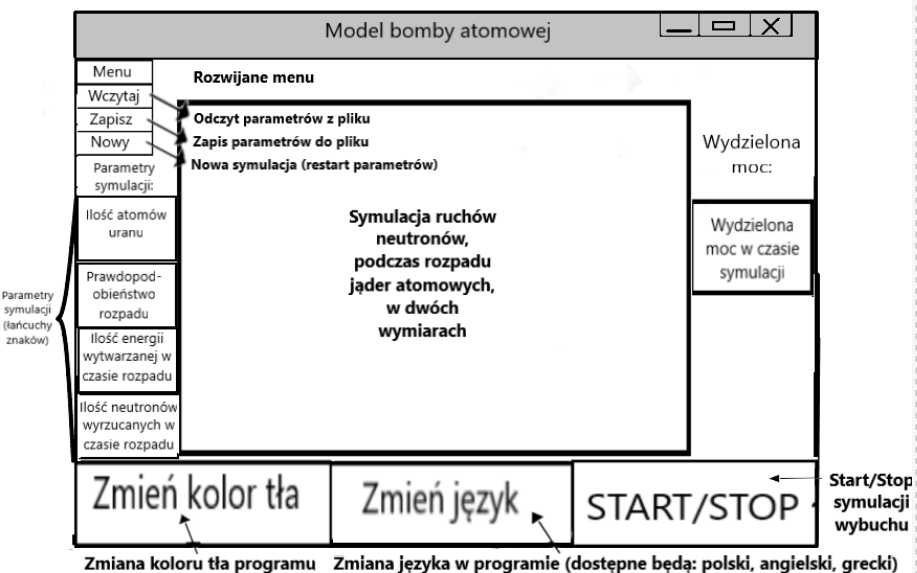
\includegraphics[scale=0.3]{GUI.png}
    \caption{Szkic GUI głównego okna programu}
    \label{fig:my_label}
\end{figure}
\section{Scenariusze użycia}
Scenariusz: Symulacja wybuchu bomby atomowej
\begin{enumerate}
    \item Ustawienie, opisanych powyżej, parametrów wybuchu.
    \begin{enumerate}
        \item Poprzez wczytanie z pliku (Menu $\rightarrow$ Wczytaj)
        \item Poprzez wpisanie string’ów w odpowiednie okienka. Będzie możliwe wybranie jednostki fizycznej, która będzie reprezentować wartość wespół z wpisaną liczbą. 
    \end{enumerate}
    \item Włączenie symulacji następuje po naciśnięciu przycisku START. Zatrzymanie z kolei po naciśnięciu przycisku STOP, który zastąpi przycisk START, gdy symulacja będzie działała. 
    \item (opcjonalnie) Wybór kolorów tła animacji oraz poszczególnych typów cząstek.  
    \item (opcjonalnie) Zapisanie wykonanej symulacji poprzez wybranie Menu $\rightarrow$  Zapisz... 
    \item (opcjonalnie) Wyczyszczenie wszystkich danych poprzez wybranie Menu $\rightarrow$  Nowy… 
\end{enumerate}
\section{Wymagania dodatkowe}
\begin{enumerate}
     \item Umieszczenie finalnego programu na serwerze w systemie kontroli wersji GIT  
    \item Użycie systemu kontroli wersji GIT podczas pisania projektu 
    \item Możliwy odczyt i zapis z(do) pliku tekstowego. 
    \item Program można zainstalować za pomocą java web start  
    \item Program można zainstalować za pomocą instalatora w systemie Windows 
    \item Skorzystanie z technik/bibliotek nie omawianych na wykładzie  
    \item Projekt jest dostępny na licencji open source.
    \item Program dostępny jest w angielskiej i polskiej wersji językowej.
\end{enumerate}

\section{Terminarz realizacji projektu}
\begin{enumerate}[label=\Roman*.]
    \item Specyfikacja (3 zajęcia)  20.III.2020 r. 
    \item Prototype - User Interface  - gotowy interfejs użytkownika - 3.IV.2020 r.
    \item Release Candidate (10 zajęcia) - implementacja minimum połowy funkcjonalności
    \item Final (15 zajęcia) - ukończony projekt spełniający założone wymagania
\end{enumerate}

\section{Ocena oraz tabela zadań}
\begin{table}
\begin{tabular}{|l|l|l|l|}
\hline
Funkcjonalność & Maksymalna ilość punktów                                                                                  & Uzyskana ilość punktów & Notatki \\ \hline
1              & GUI                                                                                                       & ….  pkt                &         \\ \hline
2              & Program znajduje się repozytorium GIT                                                                     & obowiązkowo            &         \\ \hline
3              & \begin{tabular}[c]{@{}l@{}}Poprawne zastosowanie teorii fizycznej\\ do wykonywanych obliczeń\end{tabular} & ….  pkt                &         \\ \hline
4              & Podstawowa funkcjonalność programu                                                                        & ….  pkt                &         \\ \hline
5              & System kontroli wersji GIT                                                                                & ….  pkt                &         \\ \hline
6              & Możliwa instalacja za pomocą Java web start                                                               & ….  pkt                &         \\ \hline
7              & Zapis i odczyt parametrów z pliku tekstowego                                                              & ….  pkt                &         \\ \hline
8              & Działający przycisk START/STOP                                                                            & ….  pkt                &         \\ \hline
9              & Płynna animacja wybuchu                                                                                   & ….  pkt                &         \\ \hline
10             & Angielska wersja językowa                                                                                 & ….  pkt                &         \\ \hline
11             & Umieszczona informacja o licencji programu                                                                & ….  pkt                &         \\ \hline
12             & Użycie biblioteki nie omawianej na wykładzie                                                              & … pkt                  &         \\ \hline
               & Ilość punktów:                                                                                            & ….. pkt                &         \\ \hline
\end{tabular}
\end{table}

Za poprawnie wykonany projekt chcielibyśmy uzyskać ocenę 5.

\end{document}
